%!TEX root = ../thesis.tex
%*******************************************************************************
%****************************** Third Chapter **********************************
%*******************************************************************************
\chapter{The Short-Baseline Near Detector and Booster Neutrino Beam}
\label{ChapterDetector}
% **************************** Define Graphics Path **************************
\ifpdf
    \graphicspath{{Chapter4/Figs/Raster/}{Chapter4/Figs/PDF/}{Chapter4/Figs/}}
\else
    \graphicspath{{Chapter4/Figs/Vector/}{Chapter4/Figs/}}
\fi

%********************************** %Opening  **************************************

The Short-Baseline Near Detector (SBND) is the near detector of the Short-Baseline Neutrino (SBN) program at Fermilab.
The program is motivated by anomalous results observed across various detectors involving accelerator, nuclear reactor, and solar neutrino experiments.
For instance, the low energy excess in the $\nu_e$ and $\overline{\nu}_e$ interaction measurement observed by both LSND and MiniBooNE experiments is an outstanding anomaly for the past decade \cite{LSND_anomaly, Miniboone_anomaly}.
In addition to being part of the SBN program, SBND also has its own extensive physics program focusing on high precision $\nu$-Ar cross section measurements and physics beyond the Standard Model. 
This will not only benefit future long baseline neutrino experiments such as the DUNE but also significantly advance the field of neutrino physics as a whole.
At the time of writing, SBND has entered its commissioning phase, in preparation for calibration and physics data taking.

This chapter contains an overview of the SBND detector and the Booster Neutrino Beam (BNB), which are the detector and beam source used in the search for Heavy Neutral Leptons (HNLs) in this thesis.
The chapter begins with a discussion on the physics program of the SBND experiment in Section \ref{sec4PhysicsProgram}. 
Section \ref{sec4SBND} provides a detailed description of the detection technology of SBND, covering the time projection chamber, photon detection system, and cosmic ray tagger system. 
This section also elaborates on the hardware triggering system and the data acquisition system employed at SBND.
Finally, an overview of the BNB is presented in Section \ref{sec4BNB}, detailing the particle production process of the beam and the flux prediction at SBND.
Finally, Sec \ref{sec:sbnd_conclude} provides some concluding remarks.  

%********************************** %First Section  **************************************
\section{The Short-Baseline Near Detector Physics Program}
\label{sec4PhysicsProgram}
%SBN Program

%0: SBND, as part of the SBN Program
%Neutrino Oscillation
SBND is part of the Short-Baseline Neutrino (SBN) program located at Fermilab \cite{SBNProgram}. 
The program consists of three Liquid Argon Time Projection Chamber (LArTPC) detectors: SBND, MicroBooNE, and ICARUS, positioned at distances of 110 m, 470 m, and 600 m on-axis to the target of the BNB as shown in Fig. \ref{fig:SBN_program}.
The near-far detector setup was designed to search for the potential existence of sterile neutrinos in the mass $\mathcal{O}$(1 eV) that is briefly mentioned in Chapter \ref{ChapterHNL}, driven by a series of anomalies observed by previous short baseline experiments.

Amongst these earlier experiments was the LSND experiment which utilised a stopping pion source to probe $\overline{\nu}_{e}$ via inverse $\beta$-decay and reported an excess of signal to the background at low energies with a 3.8$\sigma$ level \cite{LSND_anomaly}. 
The MiniBooNE experiment was a neutrino accelerator experiment designed to measure the entire phase space covered by the LSND result \cite{Miniboone_anomaly}.
This detector observed an excess of $\nu_{e}$ ($\overline{\nu}_{e}$) in $\nu_{\mu}$ ($\overline{\nu}_{\mu}$) beam mode showing a discrepancy from the SM with a significance level of 4.5$\sigma$ (2.8$\sigma$), reaching 6.0$\sigma$ when combined with the LSND data.
Additionally, a re-evaluation of results from the nuclear reactor experiments indicated a deficit of $\overline{\nu}_{e}$ fluxes to the theoretical expectation at a 3$\sigma$ level \cite{reactor_anomaly_1, reactor_anomaly_2}. 
%and spectral features consistent with an eV-scale sterile neutrino addition \cite{reactor_anomaly_3, reactor_anomaly_4}.
Furthermore, gallium solar neutrino experiments observed an overall deficit in $\nu_{e}$ fluxes at a 3$\sigma$ level during calibrations using radioactive neutrino sources \cite{galium_anomaly_1, galium_anomaly_2}.
These main anomalous results collectively suggest the mass mixing of SM neutrinos with an addition eV-scale sterile neutrino at a short baseline to energy ratio of $L/E \approx 1 $ m/MeV.
This can enhance or reduce the number of observed neutrino interactions for a given channel \cite{SBNProgram}.
The goal of the SBN program is to pioneer the search for eV-scale sterile neutrino oscillations, covering the parameter phase space previously allowed by past experiments but at a significance level of $\geq 5 \sigma$.

\begin{figure}[htbp] 
\centering    
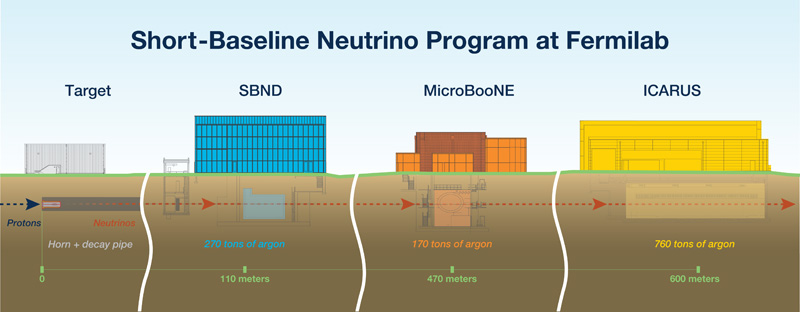
\includegraphics[width=1.0\textwidth]{SBN_program}
\caption[Short-Baseline Neutrino Program]{
Graphic showing the three LArTPC detectors made up the Short-Baseline Neutrino program: SBND, MicroBooNE and ICARUS \cite{SBNProgram}.
}
\label{fig:SBN_program}
\end{figure}

%Neutrino Cross Section
Additionally, precise measurements of $\nu$-Ar interactions play a crucial role in the physics program of SBND, serving as a critical element in understanding neutrino oscillations \cite{NuSTECWhitePaper}. 
Being the nearest to the beam target, SBND is presented with a unique opportunity to observe the largest unoscillated neutrino fluxes among the three detectors.
Over the 3-year operational span, SBND aims to record a staggering 10 million neutrino events, originating from an exposure of $1 \times 10^{21}$ Protons On Target (POT) \cite{SBNProgram}.
This will establish SBND as the world leader in statistics for $\nu$-Ar cross section measurements.
More than 6 million Charged Current (CC) $\nu_{\mu}$ events will be collected, reducing the statistical uncertainty to well below the percent level.
Moreover, SBND is expected to record 45,000 CC $\nu_{e}$ events, providing the most extensive statistics for both inclusive and exclusive measurements of this channel.
These measurements will be extremely beneficial for advancing the objectives of the SBN physics program, as well as contributing to the physics goals of the long baseline DUNE experiment, which employs argon as its detector medium.

Finally, a key aspect of the physics program at SBND is the exploration of new scenarios leading to Beyond Standard Model (BSM) physics. 
Proximity to a high intensity beam and the resulting large statistics enable searches for very weakly coupled interactions coming from the BNB \cite{SBNProgram}.
%HNL
A key example is HNLs, the primary focus of this thesis.
These can be produced from meson decays in the BNB and subsequently decay in flight into SM observables for detection (See Chapter \ref{ChapterHNL}).
%Light Dark Matter
Another compelling BSM candidate is light dark matter, which can be produced from neutral meson decay or proton bremsstrahlung \cite{LightDarkMatter}. 
%As postulated by thermal relic models, these light dark matter particles could reach sub-GeV-scale masses. 
The particles may scatter and decay, resulting in electromagnetic showers without any hadronic activities inside SBND.
%Dark neutrino
Moreover, the dynamic mass mechanism of SM neutrinos opens avenues for new physics in the dark sector. 
The dark neutrino model proposes that right-handed neutrinos can scatter with nuclei to produce dark gauge bosons, subsequently decaying into di-lepton pairs \cite{DarkNeutrino}. 
In the case where the leptons are electrons, this could potentially explain the low energy excess anomalies observed by LSND and MiniBooNE \cite{DarkNeutrinoLEE}.
These represent just a few examples of the diverse BSM scenarios that can be explored at SBND. 
Other unmentioned possibilities such as new interactions, extra dimensions, and violations of Lorentz and charge parity time symmetries, among others, contribute to the rich physics program of SBND \cite{SBNProgram}.

%********************************** %First Section  **************************************
\section{The Short-Baseline Near Detector}
\label{sec4SBND}

The SBND detector is a LArTPC with an active volume of 112 tons and dimensions of 400 cm (x-drift) $\times$ 400 cm (y-height) $\times$ 500 cm (z-length) \cite{SBNProposal}.
As depicted in Fig. \ref{fig:SBND_Pretty}, the detector consists of two separate TPCs, each with a drift length of 200 cm, sharing a common Cathode Plane Assembly (CPA) positioned at the centre.
On the east and west side of the detector are the Anode Plane Assemblies (APAs) made up of three wire planes, and located behind the wires is the Photon Detection System (PDS).
%Additionally, the PDS incorporates a passive component consisting of TPB-coated reflective foils installed at the CPA.
The TPCs are surrounded by a field cage that provides a uniform electric field.
The entire detector is placed inside a membrane cryostat, surrounded by 7 walls of Cosmic Ray Tagger (CRT) modules to provide a 4$\pi$ solid angle coverage for cosmic ray rejection.
The following sections provide an overview of each of the main subsystems of SBND.

\begin{figure}[htbp] 
\centering    
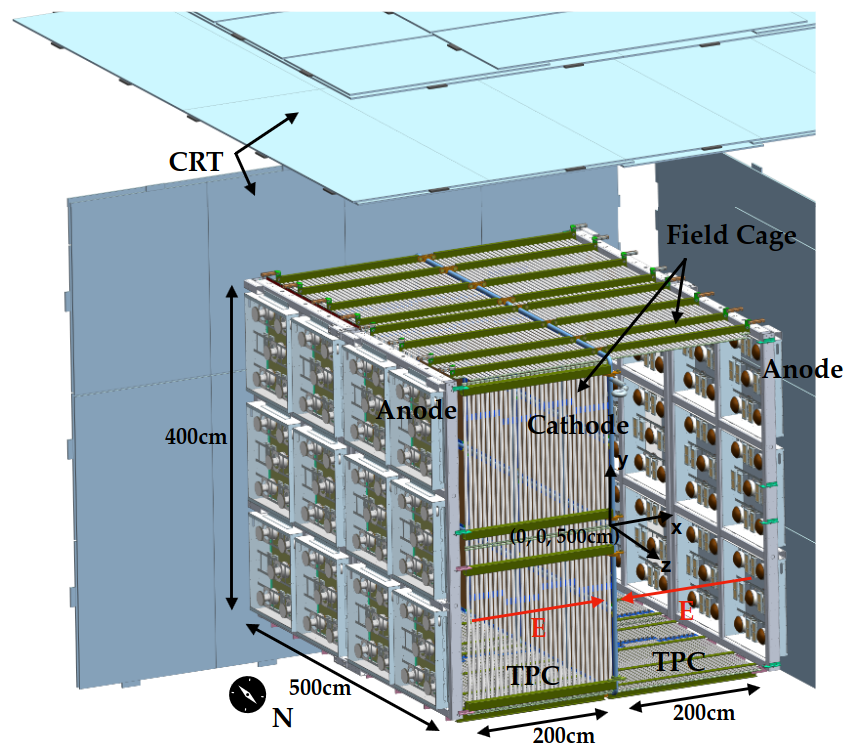
\includegraphics[width=0.9\textwidth]{SBND_Pretty}
\caption[Short-Baseline Near Detector 3D Model]{
3D model of the SBND detector, showing the LArTPC surrounded by 4 out of the 7 CRT walls \cite{sbnd_pds_paper}. 
}
\label{fig:SBND_Pretty}
\end{figure}

\subsection{Time Projection Chamber}

Fig. \ref{fig:SBND_APA_diag} shows a complete APAs, of which each plane of APAs is located on the east and west sides of SBND.
The plane is made up of two coupled APAs, where an APA measures 4 m $\times$ 2.5 m and comprises a steel frame supporting three wire planes: two induction planes, denoted as U and V, oriented at angles of $\pm 60^{\circ}$ to the vertical collection plane denoted as Y. 
These wire planes U, V and Y are colour-coded as green, blue, and red, respectively.
Each wire plane is constructed with 150 $\mu$m diameter copper-beryllium wires, with a wire pitch and plane spacing of 3 mm. 
The wires are tensioned to 7 N to prevent slackening when cooled down to a temperature at 88.4 K \cite{SBND_Wires}.
To maintain charge transparency for the induction planes and collection efficiency for the collection plane, a biased voltage of -200 V, 0 V, and 500 V is applied to planes U, V, and Y, respectively.
In total, each TPC consists of 5,632 wires: 1,664 wires in the collection plane and 1,986 wires in each induction plane.

Two APAs are coupled together utilising jumper cables to bridge the 15 mm gap between the induction planes to form a single electronic channel. 
Attached to the top, left and right side of APAs are the cold electronics readout boards.
They pre-amplify and digitise wire signals while submerged in liquid argon at a low temperature to minimise noise. 
Fig. \ref{fig:SBND_APA} shows a photograph of a fully assembled APAs at SBND, where the PDS located behind the wires can also be seen.  

\begin{figure}[hb!] 
\centering    
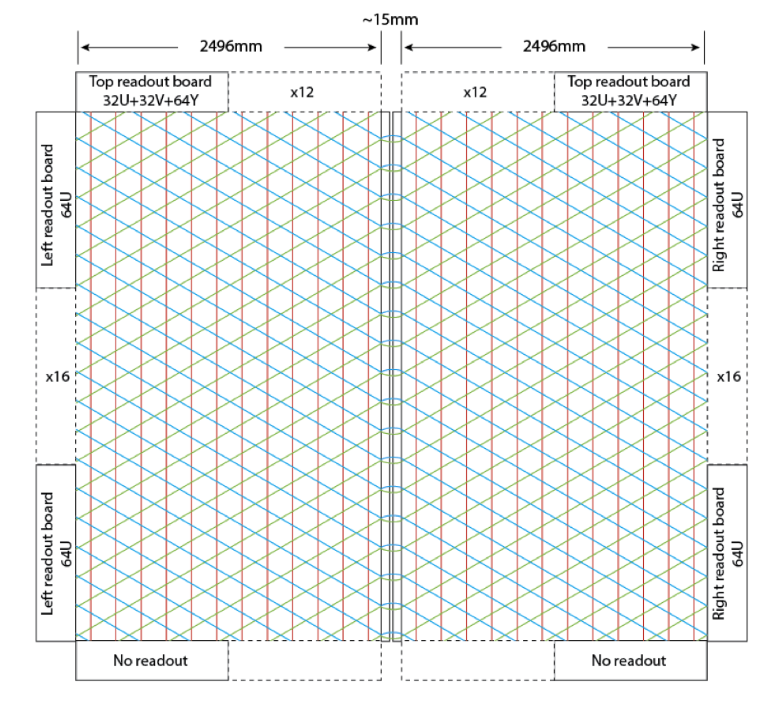
\includegraphics[width=0.65\textwidth]{SBND_APA}
\caption[Anode Plane Assemblies Schematic]{
Schematic showing two coupled APAs to form a complete APAs \cite{SBNProposal}.
}
\label{fig:SBND_APA_diag}
\end{figure}

Fig. \ref{fig:SBND_CPA} shows a photograph of the fully assembled CPA.                                                                                                                                 
The plane consists of two steel frames, each containing 8 windows, adding to a total of 16 windows.
Each window, measuring 60 cm $\times$ 50 cm, houses a fibreglass plate laminated on both sides with non-conductive reflective foils of $> 99\%$ specular reflection in the visible range and coated with TetraPhenyl Butadiene (TPB).
Furthermore, the plate is covered by a wire mesh, providing a high voltage at -100 kV supplied by a feedthrough donut from outside the cryostat.

%Field Cage
The field cage consists of a sequence of electrodes arranged perpendicular to the drift direction.
It can be seen in both Fig. \ref{fig:SBND_APA} and \ref{fig:SBND_CPA} as the series of metal bars surrounding the TPC.
These electrodes incrementally step up the voltage from -100 kV applied at the CPA to the ground voltage in steps of 3 kV. 
This gradual voltage increase is implemented to maintain a uniform electric field of 500 V/cm across the drift volume.

\begin{figure}[htbp!]
%\hfill
\begin{subfigure}[h]{0.5\linewidth}
\centering    
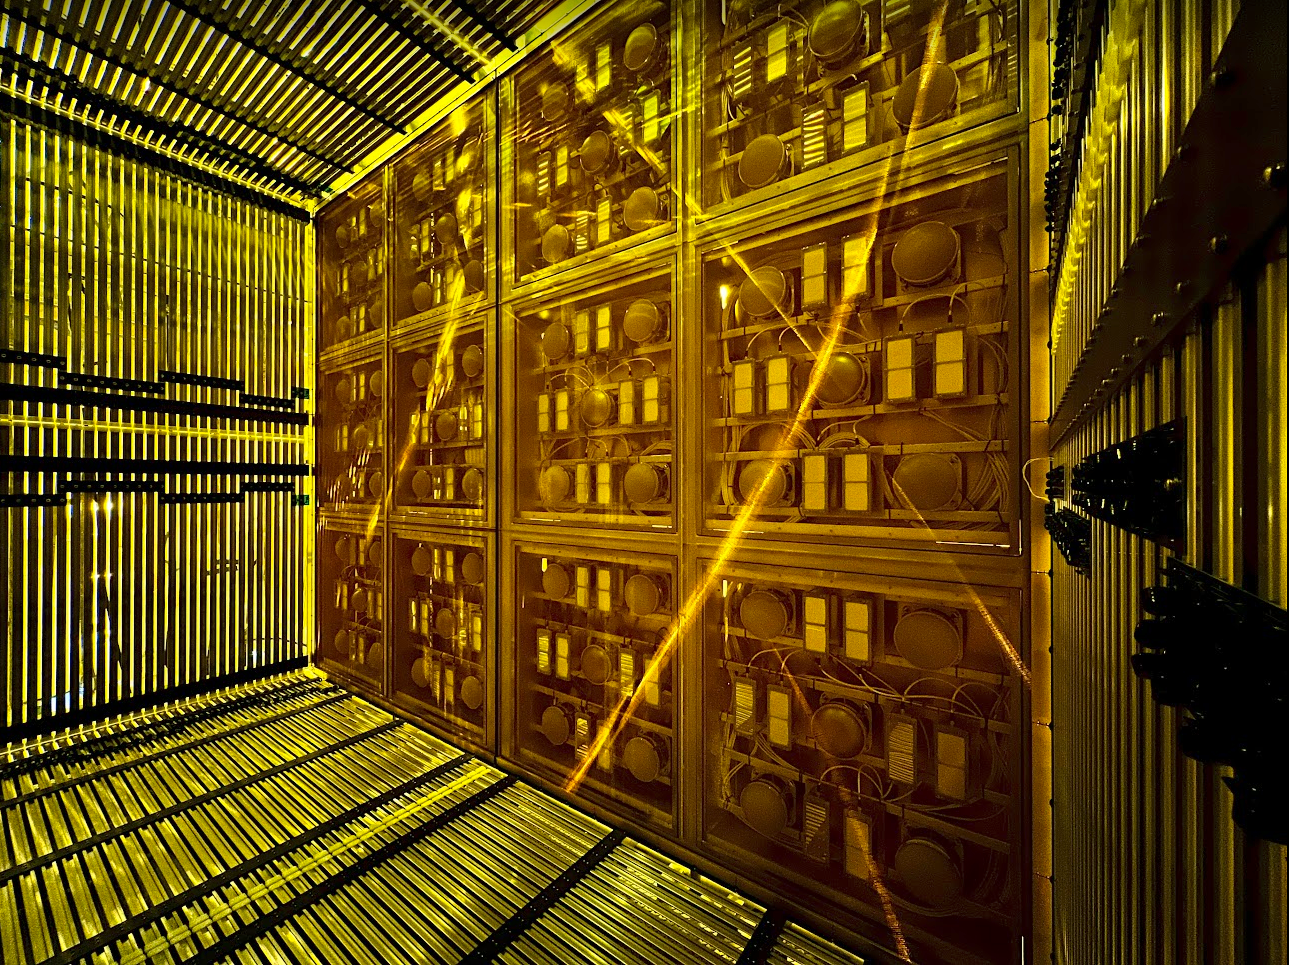
\includegraphics[width=\linewidth]{SBND_APA_PDS}
\caption{View of the APA}
\label{fig:SBND_APA}
\end{subfigure}%
\hfill
\begin{subfigure}[h]{0.5\linewidth}
\centering    
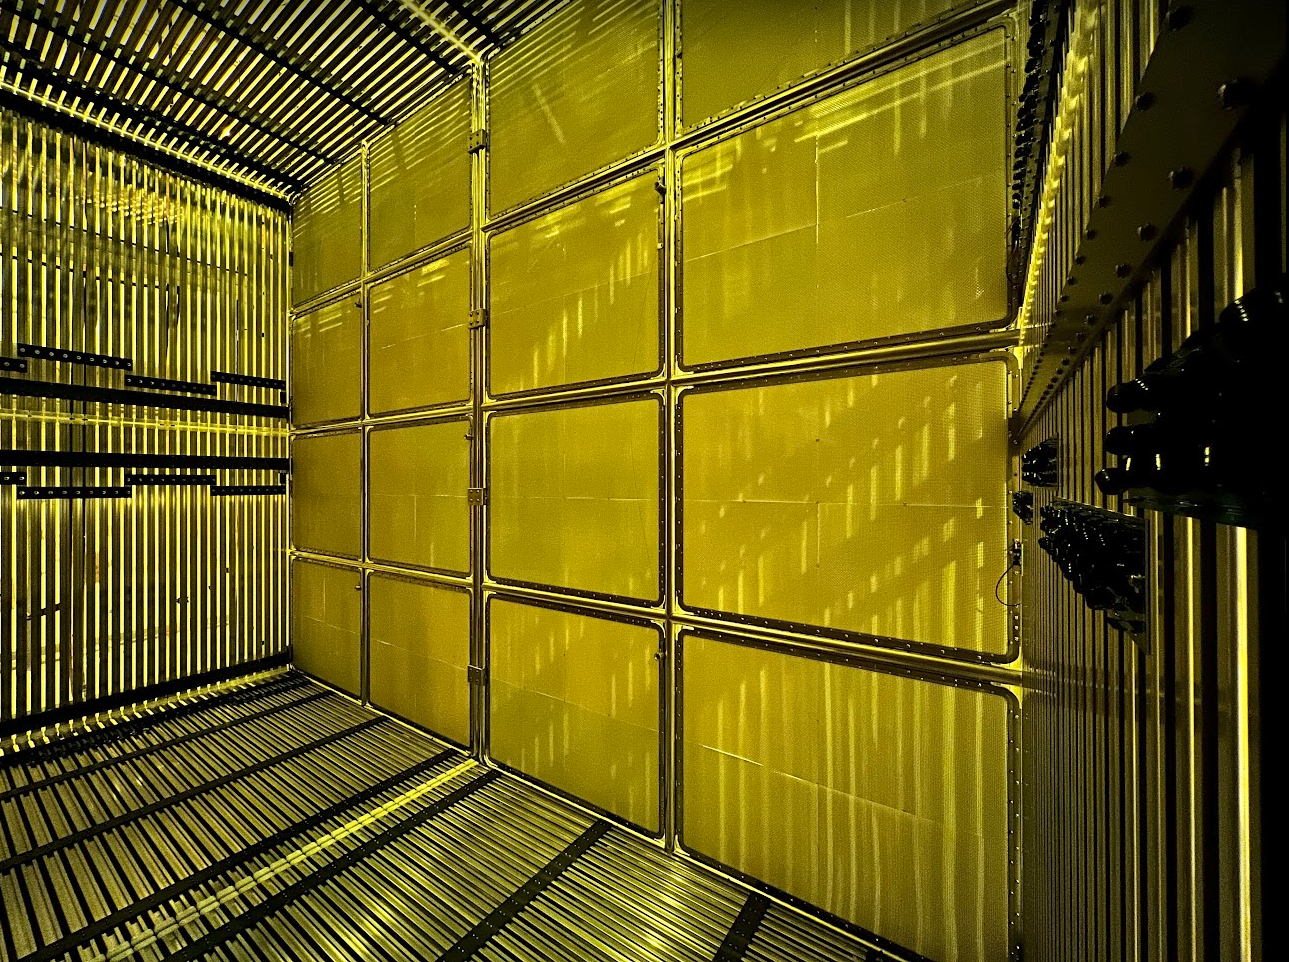
\includegraphics[width=\linewidth]{SBND_CPA}
\caption{View of the CPA}
\label{fig:SBND_CPA}
\end{subfigure}
\caption[Time Projection Chamber Photographs]{
Photographs showing the fully assembled TPC of the SBND detector. 
}
\label{fig:SBND_CPA_APA}
\end{figure}

\subsection{Photon Detection System}
\label{sec:sbnd_pds}

%describe PMT, XARAPUCA and TPB
The PDS design of SBND is the most sophisticated system ever installed in a LArTPC, by incorporating both active and passive optical components \cite{sbnd_pds_paper}. 
The active optical detector integrates two different technologies: (1) 120 Photomultiplier Tubes (PMTs) and (2) 192 X-ARAPUCA devices.
The PMTs are cryogenic 8"-diameter Hamamatsu R5912-MOD models \cite{hamamatsu}, which are the primary light detection system. 
Meanwhile, the X-ARAPUCAs serve as a research and development platform for future experiments, incorporating multiple variations in their components for performance comparison. 
A summary of the X-ARAPUCA specifications can be found in Ref. \cite{sbnd_pds_paper}.
The TPB-coated reflective foils installed at the CPA are the passive component to improve the uniformity of light yield.

%PDS Box
Fig. \ref{fig:SBND_PDS} shows a 3D model for each component of the SBND PDS.
For the purpose of installation, the optical detectors are arranged into modular PDS boxes, of which a single PDS box is shown on the left of Fig. \ref{fig:SBND_PDS}.
Each box houses 5 PMTs, 4 coated and 1 uncoated PMT, along with 8 X-ARAPUCA devices, 4 coated and 4 uncoated.
These PDS boxes are installed in a configuration of $4 \times 3$ behind each APAs as illustrated on the right of Fig. \ref{fig:SBND_PDS}.
This results in a total of 12 boxes per TPC volume.
The TPB-coated reflective foils at the central cathode can also be seen on the right of Fig. \ref{fig:SBND_PDS}.

\begin{figure}[hbp]
\centering    
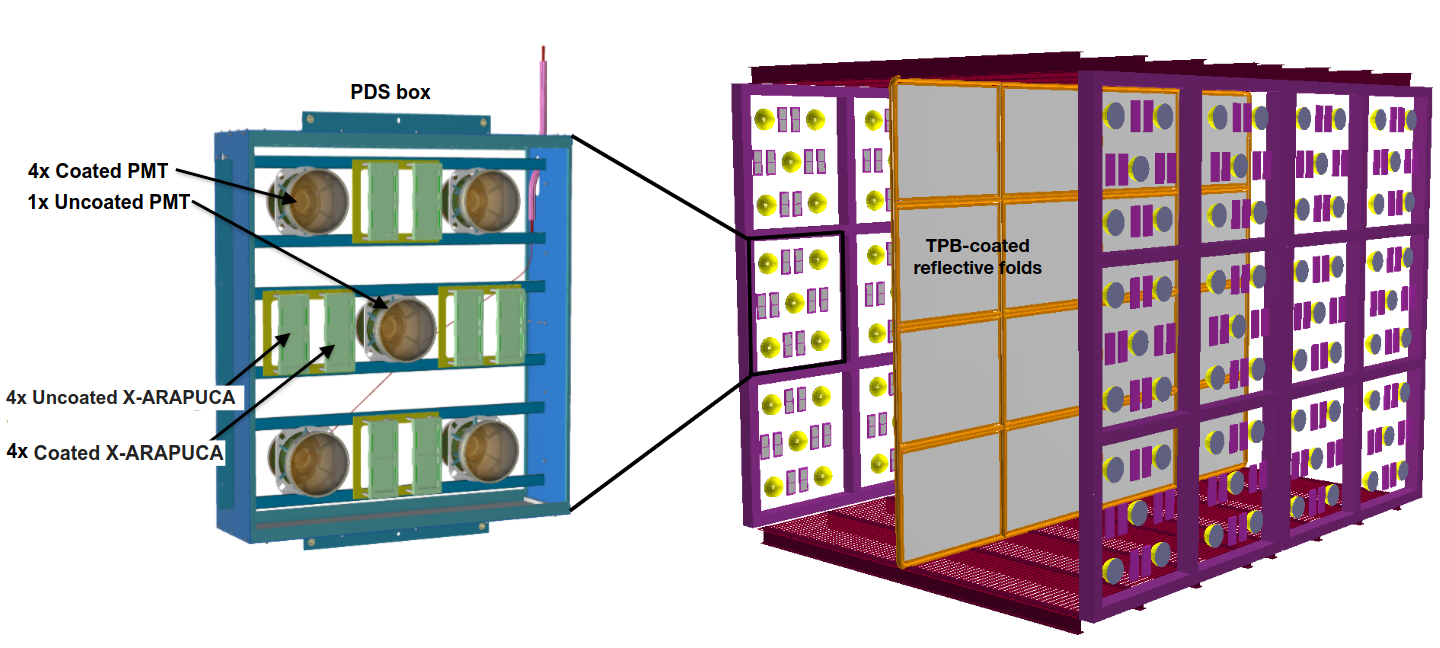
\includegraphics[width=0.85\textwidth]{SBND_PDS}
\caption[Photon Detection System 3D Model]{
3D model of a PDS box (left) and the PDS box arrangement on the east and west side of the TPC (right) \cite{sbnd_pds_paper}.
}
\label{fig:SBND_PDS}
\end{figure}

Out of the two optical detectors, PMT signals are the primary light signals and are used to provide trigger conditions.
The 120 PMTs are partitioned into two optically-isolated TPC volumes, each with 60 PMTs.
Within each TPC, 48 PMTs are TPB-coated, and thus are sensitive to both direct VUV and reflected visible light, while the remaining 12 non-coated PMTs detect only reflected light. 
This ratio of coated to uncoated PMTs (4:1) is chosen to optimize light collection efficiency while maintaining the capability to distinguish between the two light components \cite{sbnd_pds_paper}. 

Having TPB is utilised at two locations: (1) evaporated onto reflective foils at the cathode, and (2) coated on the optical windows of the PMTs, leads to a difference in the spatial and arrival time distributions for direct VUV and reflected visible photons.
Direct VUV photons arriving at coated PMTs are immediately wavelength shifted into the detectable range of PMTs.
Reflected visible photons, resulting from VUV photons being wavelength shifted and reflected at the cathode, have to travel a longer distance before being detected by uncoated PMTs.
The spatial distribution of reflected visible photons is more diffused and spread across a larger number of optical detectors compared to direct VUV photons \cite{PatrickPhD}.
%However, reflected visible photons have a faster group velocity (See Fig. \ref{fig:vuv_visible} Section \ref{sec:photonprop}) and arrive at detection earlier than some direct VUV photons.
Such difference can be exploited to perform the timing reconstruction using only PMT signals, which is further discussed in Section \ref{sec:reco_pds}.

\subsection{Cosmic Ray Tagger}
\label{sec:sbnd_crt}

Since SBND is a surface detector, it utilises a Cosmic Ray Tagger (CRT) system to effectively reject background from cosmic muons.
Fig. \ref{fig:SBND_CRT} shows the operating principles of CRT strips and their orientation \cite{RhiannonPhD}.
As shown in the middle diagram, each CRT strip consists of a plastic scintillator strip with a width of 10.8 cm, connected to a pair of SiPMs via wavelength shifting optical fibres.       
The right diagram shows a coincident hit from perpendicular strips that allows for a 2D reconstruction of the hit location, and the number of photons collected for each strip improves the precision of the location tagging.
\begin{figure}[b!] 
\centering    
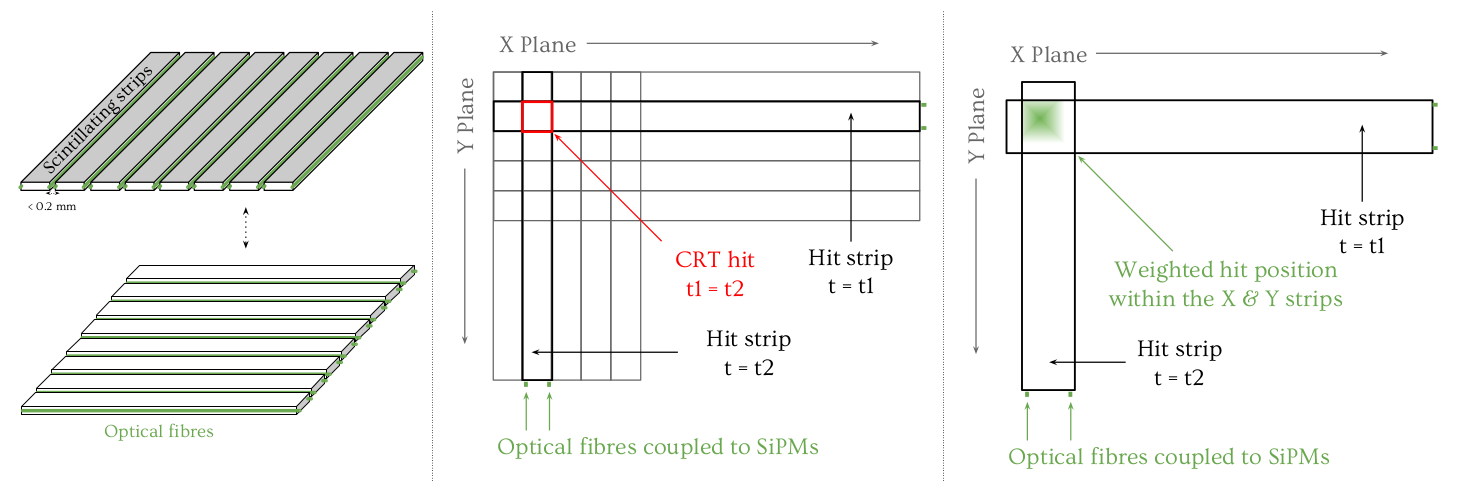
\includegraphics[width=1.0\textwidth]{SBND_CRT}
\caption[Cosmic Ray Tagger Diagrams]{
Diagrams showing the operating principles of CRT strips (middle, right) and their perpendicular orientation (left) \cite{RhiannonPhD}.
}
\label{fig:SBND_CRT}
\end{figure}

The left diagram of Fig. \ref{fig:SBND_CRT} shows an example of 8 CRT strips arranged in parallel to form a CRT module and the modules are perpendicular to each other.
Multiple CRT modules are arranged orthogonally to form a CRT wall, typically in the size of 7.5 m in height and 9 m in width.
The cryostat of SBND is entirely encased by 7 CRT walls, with 1 on each side and 2 positioned on top of the detector.
Fig. \ref{fig:SBND_Pretty} shows 4 out of the 7 CRT walls, particularly the south, west and top walls are visible.
Additionally, the top 2 walls function as a cosmic telescope, facilitating the tagging of vertical downward going cosmic muons.
This configuration enables a comprehensive strategy for cosmic background rejection utilising both geometrical and high precision timing information.
%For instance, tracks identified by the TPC can be matched to CRT hits to identify tracks occurring outside the beam spill window.
%Signals from the SiPMs are amplified, digitised and read out by the Front End Board (FEB) modules with nanosecond timing resolution, which will be detailed in Section \ref{}. 

\subsection{Readout Electronics}
\label{sec:readout}

%Cold Electronic
The readout electronics of each detection subsystem are detailed next.
Firstly, TPC readouts comprise four components: (1) Cold Electronics (CE), (2) Warm Interface Boards (WIBs), (3) TPC crates and (4) Nevis Trigger Board (NTB).%, shown as the red boxes from left to right respectively in Fig. \ref{fig:daqOverview}.
As shown in Fig. \ref{fig:SBND_APA_diag}, the wires are connected to CE readout boards on the APAs.
Located inside the cryostat, CE are submerged in liquid argon to reduce thermal noise as well as cable lengths \cite{SBND_CE}.
They amplify and digitise signals at a sampling frequency of 2 MHz. 
Data from CE is sent outside of the cryostat to the WIBs via copper cold cables.              
The WIBs are connected to other TPC readouts through optical fibre links.
This isolation architecture completely separates wire grounding from the building, thereby enabling a superior signal-to-noise ratio.

%Nevis Readout
Following the WIBs, data is transmitted to 11 TPC crates for reading out, buffering, and processing the wire signals. 
Data from TPC crates are directed by the NTB into two parallel independent streams of data.
%The main stream to record neutrino beam events relies on the ETRIG trigger signal from the PTB for triggering as previously detailed in Section \ref{sec:sbnd_trigger}, which reads out data with lossless compression.
The main stream to record neutrino beam events relies on an external trigger, which reads out data with lossless compression.
An additional continuous stream requires no external triggers and outputs data with lossy compression. 

%CAEN digitiser
Regarding the readout electronics of the PDS, CAEN digitisers are employed. % depicted as the blue boxes in Fig. \ref{fig:daqOverview}
120 PMTs are readout by 8 CAEN V1730SB digitisers \cite{caen1730}, capable of recording waveforms for 16 channels independently with a sampling frequency of 500 MHz.
192 X-ARAPUCAs are digitised by another model called V1740 \cite{caen1740}, that can readout 64 channels at a lower sampling frequency of 62.5 MHz.
Both models feature deep buffers to store longer waveforms and handle higher data rates.
Additionally, the V1730SB model offers better waveform baseline stability against temperature fluctuations.
Multiple CAEN digitisers can be synchronised so that they collectively behave as a single digitiser, which is critical to maintaining the timing resolution of the electronics $\mathcal{O}$(1 ns).
The characterisation of synchronisation across multiple V1730SB digitisers is detailed in Section \ref{sec4PMT}.

%The timing resolution of the CRT readout electronics is evaluated in the following section.
%CRT FEB
Finally, 7 CRT walls are readout by 144 Front End Board (FEB) modules \cite{crt_note}.%, as shown by the orange box in Fig. \ref{fig:daqOverview}.
Each module is a multifunctional board capable of reading out 32 channels, with one channel per SiPM. 
The module provides a bias voltage, adjustable for individual SiPMs, as well as signal amplification and shaping.
Once the signal is shaped, the module applies signal discrimination and self-triggering, such as coincidence for each pair of SiPMs in a CRT strip or coincidence across multiple modules for orthogonal CRT strips. 
Once the signal passes the self-trigger, it is digitised and timestamped with respect to an input reference clock. 
The data is stored in a buffer and sent via an Ethernet connection. 
The characterisation of the timing resolution of FEB modules is detailed in Section \ref{sec4InternalClock}
%The following section focuses on the characterisation on the timing resolution of the FEB module.

\subsection{Hardware Trigger}
\label{sec:sbnd_trigger}

Triggering plays a vital role in the SBND detector to select only interesting physics events, given the detector is exposed to a high rate of backgrounds from cosmic muons. 
The main hardware trigger component in SBND is the Penn Trigger Board (PTB).
It applies a programmable trigger logic based on external inputs and issues a trigger to the Data Acquisition (DAQ) subsystem if the conditions are met.
Details of the hardware trigger at SBND is given in Appendix \ref{appendix_hardware_trigger}, while a short summary is provided here.

In order to form a trigger, the PTB requires signals from the three subsystems: (1) beam system, (2) PMTs, and (3) CRTs.
The beam system informs the PTB on the status on the BNB beam, and whether the beam has arrived at the detector hall.
Signals from PMTs provides information regarding the intensity and locality of the energy deposited inside the detector, and whether it is consistent with a neutrino event.
Signals from CRTs provides information of the energy deposited outside of the detector in the CRT walls, and whether it is consistent with a cosmic muon. 
The readout electronics of PMTs and CRTs are equipped with timing resolution $\mathcal{O}$(2 ns) and their output signals can quickly inform the PTB to form a trigger.
Additionally, incorporating CRT signals marks SBND as the first instance of a LArTPC to employ CRTs as part of its triggering scheme \cite{CPAD2022}.

Different combinations of signal inputs described here can form different \textit{flavours} of triggers.
%The primary beam trigger requires majority triggers from PMTS and threshold crossings from MTC/A to coincide with the beam early warning signal.
The primary \textit{beam} trigger requires PMT signals to coincide with the beam spill window.
Conversely, the \textit{off-beam} trigger uses an anti-coincidence to the beam signal logic to select cosmic muons occurring outside of the beam spill window for background estimation purposes.
The \textit{calibration} trigger utilises coincidence across different CRT walls to select specific track topologies formed by cosmic muons.
For example, anode-to-cathode-crossing cosmic tracks can be selected by requiring the east and west CRT walls to be coincident.
These sets of tracks are useful for electron lifetime measurements, which is covered in Section \ref{sec7:etime}.

The importance about the hardware triggering at SBND is that a single triggered physics event constitutes of two \textit{types} of triggers: (1) a single Event TRIGger (ETRIG) issued to the TPC readouts and (2) multiple Flash TRIGgers (FTRIGs) issued to the PDS readouts.
The ETRIG is used by the DAQ to acquire a long snapshot of the TPC waveform $\mathcal{O}$(1 ms) while multiple FTRIGs are used to capture many short snapshots of optical detector waveforms $\mathcal{O}$(10 $\mu$s).
The data is then assembled to build a physics event, of which the DAQ is explained in Section \ref{sec4DAQOverview} and \ref{sec:evb} next.

\subsection{Data Acquisition}
\label{sec4DAQOverview}

Upon receiving a hardware trigger, the DAQ begins to transport data from subsystem readouts to event builder machines. 
The SBND DAQ can assemble data from each subsystem into a physics event during real time data flow, known as the event building process.
It must also be able to handle a high event rate due to the close proximity of SBND to the beam target.
Additionally, the DAQ can apply software metrics to filter events for various data streams and data monitoring purposes.

Fig. \ref{fig:daqOverview} shows the data flow of the DAQ at SBND.
It begins with raw signals from detection subsystems, shown as the coloured dotted arrows.
The signals are acquired by readout electronics, shown as colour boxes in the first column labelled \textit{Readout Electronics} (See Section \ref{sec:readout}).
The boxes are colour-coded as red, blue and orange for the TPC, PDS and CRT readout respectively.
Within this first column, two additional readout electronics are also included.
The PTB, shown by the green box, is for the hardware triggering subsystem (See Section \ref{sec:sbnd_trigger}).
The White Rabbit SPEC-TDC, shown by the purple box, is part of the White Rabbit timing subsystem and is discussed in Chapter \ref{ChapterDAQ}.

Each readout electronics has a corresponding \textit{boardreader}, shown by the second column labelled \textit{Servers Hosting Boardreaders}.
Boardreaders are software tools serving as a communication bridge between readout electronics and computer servers.
%There is a two-way communication between readout electronics and boardreaders.
The electronics send raw signals to the computer servers via boardreaders, shown as the grey dotted arrows.
The boardreaders send configurations to the electronics, shown as the grey dashed-dotted arrows.

The event building process occurs in the third column labelled \textit{Event Builder Machines}.
The raw signals are packaged into a data format known as \textit{fragments} by boardreaders.
The fragments are sent to event builders, as shown by the coloured solid arrows.
The event builders assemble fragments from different readout electronics into physics events.
The event building process is discussed in Section \ref{sec:evb} next.
                        
Finally, the fourth column labelled \textit{Data Stream} illustrates the last stage of the data flow.
Software metrics are applied by event builders to separate physics events into different streams of data, as shown by the grey dashed arrows.
This assists with data management since different flavours of triggered events can be organised into different locations.
An additional data stream for online monitoring is shown by the bottom right grey box.
Details of the data streaming process is provided in Appendix \ref{appendix_data_stream}.

\begin{figure}[ht!] 
\centering    
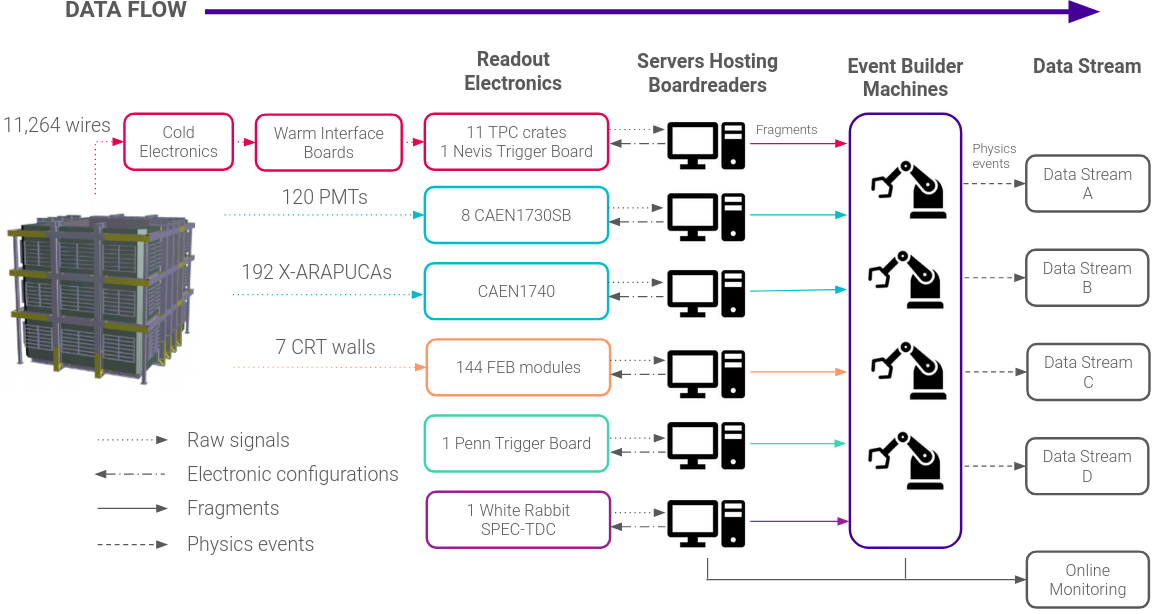
\includegraphics[width=1.0\textwidth]{DAQ_Overview}
\caption[Data Acquision Flow Chart]{
Flow chart showing the data flow of data acquisition.
}
\label{fig:daqOverview}
\end{figure}

%Each detection subsystem incorporates specialized hardware components for digitizing and reading out the physical signals. 
%The PTB, as a hardware board within the SBND trigger system, is responsible to provide triggering signals to each detection subsystem independently.
%The SPEC-TDC is a specialised timing mezzanine module designed specifically for timestamping purposes.
%Further details about its functionality are outlined in section \ref{subsec42TimeRef}.

\subsection{Event Building}
\label{sec:evb}

One key process in the DAQ is event building.
This is achieved by using the artdaq Toolkit, developed by the Real-Time Systems Engineering Department of Fermilab's Scientific Computing Division \cite{artdaq_note}. 
%This software serves as the backbone for communication between the hardware electronics and the event builder machines.
Within this framework, each readouts has a corresponding software module called \textit{boardreader}.
They facilitate communication between the readouts and the event builder machines, by sending configurations directly to the hardware in one direction and retrieving data from the hardware in the opposite direction.
Data acquired from the readouts is packaged by boardreaders into a digitised format called a \textit{fragment}.
%Technical details of boardreaders and fragments can be found in Ref. \cite{artdaq_note}.
In the scope of this work interested in the timing  performance of the DAQ to be given in Chapter \ref{ChapterDAQ}, the critical information of a fragment is its timestamp corresponding to when the readout electronics receive a trigger.

%, as depicted in Fig. \ref{fig:fragmentDiagram}. 
%The fragment class consists of a header containing experiment-specific information essential for event building, an optional metadata, and a data payload storing the hardware-defined data.
%A fragment is generated by the boardreader when its corresponding hardware readout receives a trigger.
%The timestamp of the trigger arrival is encoded as the fragment timestamp. 
%This timestamp is a crucial piece of information for the event building process.

%\begin{figure}[tbp!] 
%\centering    
%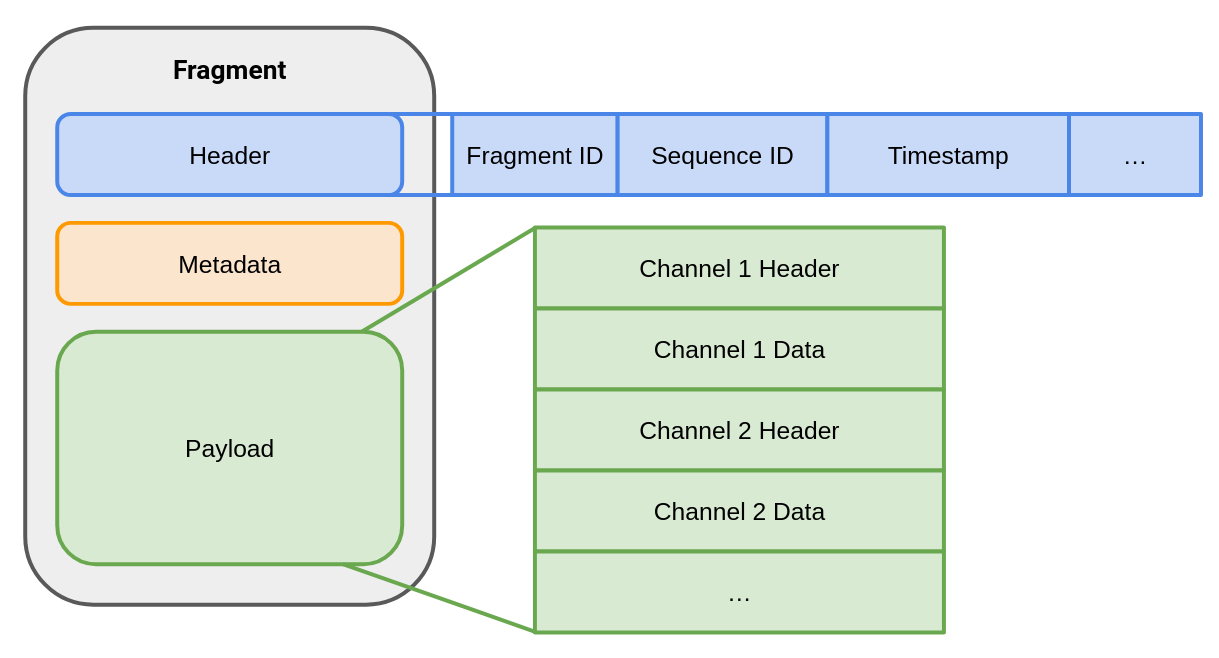
\includegraphics[width=0.6\textwidth]{Fragment_Diagram}
%\caption[FragmentDiagram]{
%Diagram illustrating the fragment class defined by the \textit{artdaq Toolkit}. 
%The header contains the crucial fragment timestamp information needed for event building.  
%%Optionally, the metadata structure contains hardware configurations. 
%%The payload is designated for storing data from the hardware readout, of which the data structure is pre-defined by the hardware. 
%}
%\label{fig:fragmentDiagram}
%\end{figure}


%what is push/pull

%Once fragments are generated, boardreaders can send them to the event builders in one of two configurations: (1) push or (2) pull.
%In the push configuration, the boardreader actively sends fragments continuously at the rate at which the fragments are generated. 
%With each fragment sent, the push boardreader also creates a request message, which is multicast to all other boardreaders currently in pull mode. 
%This request message contains the timestamp of the push fragment.
%The sequence ID of the fragments determines the sequence ID of the built event, ensuring  that every fragment is built as a single event.

%In contrast to the push configuration, the boardreader in the pull configuration stores the fragments in its buffer as they are being generated. 
%These fragments are sent to the event builders only upon receiving a request message.
%The pull boardreader checks its buffer and selects the fragments with timestamps falling within a specified time window of the request message, known as a \textit{pull window}.
%It then dispatches these selected fragments to the event builders. 
%Subsequently, the event builder machines assemble this set of pull fragments, together with the one push fragment that initially generated the request message, into a single event.
%To determine which fragments to send, the boardreader has a configurable parameter called pull window, which specifies a time window relative to the timestamp of the request message.
%The pull boardreader checks its buffer and selects the fragments with timestamps falling within this defined time window.
%The selected fragments that meet the timestamp requirement are then dispatched to the event builders.
%The sequence ID of the resulting event is determined by the push fragment.

Event builders assemble fragments from different boardreaders into a physics event based on their timestamps.
Fig. \ref{fig:SBNDEventStructure} illustrates the chronological structure of a physics event at SBND, containing only TPC, PMT and CRT fragments for simplicity.
The time axis is shown as the purple arrow, where at the centre $t = 0$ ms corresponds to when the beam spill begins.
The TPC fragment, as shown in red, is coincident with the beam spill to capture the neutrino event in the TPC. 
The readout length of a TPC fragment is 1.7 ms, covering the entire TPC drift length of 1.3 ms and including a padding of 0.2 ms before and after the drift. 
Aligning the TPC fragment with the beam spill is achieved through the ETRIG trigger issued to the TPC readouts so that the readout window coincides with when the beam spill begins.

\begin{figure}[b!] 
\centering    
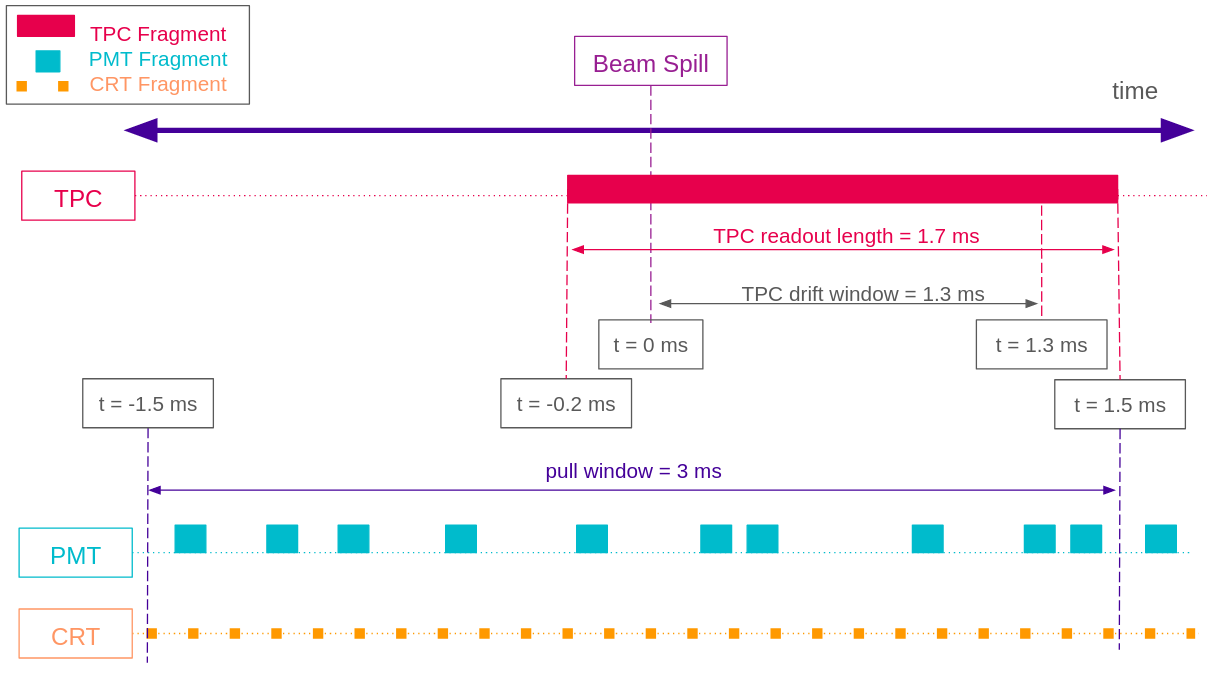
\includegraphics[width=0.85\textwidth]{SBND_Event_Structure}
\caption[Chronological Structure of a Physics Event Diagram]{
Diagram depicting the chronological structure of a physics event. 
}
\label{fig:SBNDEventStructure}
\end{figure}

%describe an event structure
%A neutrino beam event at SBND is structured as outlined in Fig. \ref{fig:SBNDEventStructure}, with examples provided for TPC, PMTs, and CRTs fragments.
%The PTB first sends a single ETRIG to the NTB that coincides with the start of the BNB beam spill if it determines a neutrino event occurs. 

%The ETRIG timestamp is encoded in the NTB fragment header.
%The NTB boardreader operates in push configuration, thus driving the data acquisitions of the PMT and CRT readouts in pull configuration.
%Within this structure, there is only one push boardreader that increments the event sequence ID counter whilst the remaining boardreaders run in pull configuration.
%The push boardreader is called the Nevis Trigger Board (NTB), which is a component of the hardware complex to readout the TPC data. 

%Meanwhile, the boardreaders for the PMTs and CRTs are in pull mode.
PMT and CRT fragments are shown in blue and orange in Fig. \ref{fig:SBNDEventStructure}.
The fragment readout lengths from the PMTs and CRTs are much shorter compared to TPC fragments, $\mathcal{O}(10\ \mu$s) and $\mathcal{O}(10$ ns) respectively.
For a single physics event, in contrast to only a single ETRIG issued to the TPC readouts, multiple FTRIGs are issued to the PMT readouts during the beam spill to produce multiple fragments of PMTs.
Similarly, CRT readouts are self-triggered independently and produce multiple fragments.
PMT and CRT fragments that have timestamps within 1.5 ms before and after the beginning of the beam spill are packaged together with the TPC fragment to form a physics event.

%The pull window is defined to be 3 ms centred on the timestamp of the NTB fragment. 
%This window includes PMT and CRT fragments generated 1.5 ms before and after the beam spill starts. 

%event asymmetry
Here in Fig. \ref{fig:SBNDEventStructure}, a time asymmetry can be seen in the chronological structure of a physics event at SBND.
This is due to the different characteristics of photon signals, detected by the CRTs and PMTs, and electron signals, detected by the TPC wires. 
Specifically, a photon produced in a CRT scintillator strip takes approximately 5 ns to travel from the far end of the strip until reaching a SiPM \cite{crt_note}. 
Similarly, a photon produced in the TPC takes a maximum of 15 ns to propagate from a scintillation location to a PMT \cite{sbnd_pds_paper}.
In contrast, an ionisation electron produced takes 1.3 ms to fully drift from the cathode to the anode \cite{SBND_Wires}.
This shows that photon signals propagate approximately six orders of magnitude faster than electron signals and consequently, need to be digitised and read out earlier.
%The time asymmetry of the event structure is due to scintillation photon signals propagating faster compared to electron signals.

%********************************** %First Section  **************************************
\section{The Booster Neutrino Beam}
\label{sec4BNB}

%Describe rate
SBND directly measures neutrino fluxes coming from the BNB.
Technical details of the BNB can be found in Ref. \cite{BNBMiniBooNE}.
The BNB operates by extracting protons with a kinetic energy of 8 GeV from the Booster synchrotron in spills made up of 7 to 11 pulses in a row at a frequency of 15 Hz, averaging to a rate of $\sim$5 Hz.
Each spill delivers $5 \times 10^{12}$ protons within a window lasting 1.6 $\mu$s.
The structure of a beam spill structure consists of 81 neutrino buckets, with a Gaussian width of 1.308 ns and a spacing of 19 ns \cite{BNBsigma}.
Fig. \ref{fig:CRT2017} depicts the beam bucket structure as measured by the CRTs of SBND, which was set up as a beam telescope to collect data from the BNB in 2017--2018 \cite{CPAD2022}.
Neutrino buckets can be seen distinctively in the distribution, indicating that the BNB structure can be resolved with a sufficient timing resolution.
The timing resolution of the CRT readouts is $\mathcal{O}$ (2 ns), to be demonstrated later in Section \ref{sec4InternalClock}.

\begin{figure}[ht!] 
\centering    
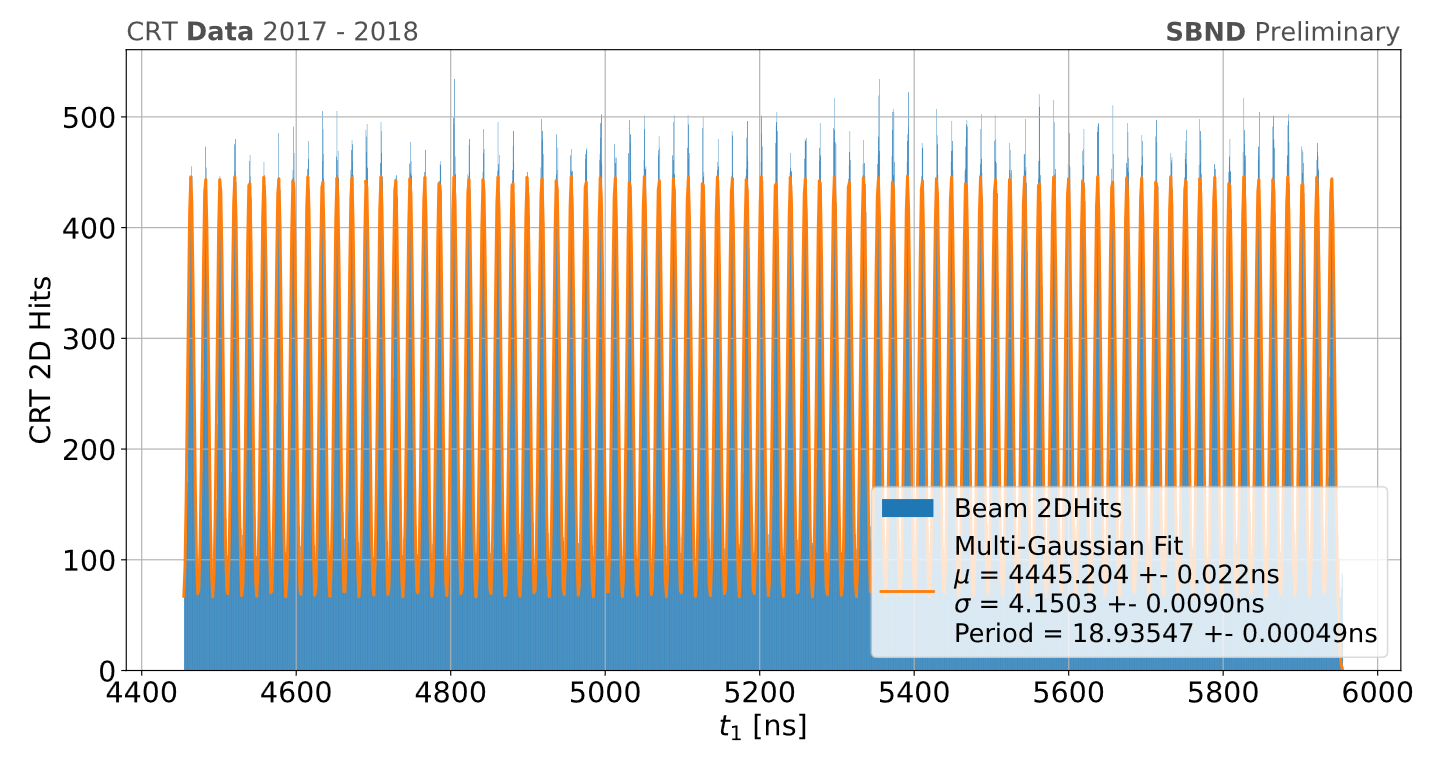
\includegraphics[width=0.85\textwidth]{CRT2017}
\caption[Booster Neutrino Beam Measured by SBND CRTs in 2017-2018]{
The buckets of the BNB measured by the SBND CRTs during 2017--2018 \cite{CPAD2022}.
}
\label{fig:CRT2017}
\end{figure}

%hardware structure
The particle production in the BNB is illustrated in Fig. \ref{fig:BNBDiagram}.
Protons are injected into the Booster synchrotron and accelerated from 400 MeV to 8 GeV kinetic energy, as shown by the red arrows. 
Their intensity is measured by two toroids, while their positioning and timing are monitored by beam position monitors and Resistive Wall Monitors (RWM) \cite{BNBRWM}.
Upon exiting the Booster, the proton beam traverses focusing and defocusing quadrupole and dipole magnets before being focused onto the target of the BNB.

The protons collide on the target to produce secondary mesons, as shown by the blue arrows.
The target consists of a beryllium cylinder measuring 71.1 cm in length and 0.51 cm in radius.
The choice of beryllium was motivated by its replaceable ability in the event of radioactivity issues, as well as its ability to facilitate sufficient energy loss via an air cooling system.
The target is placed inside a pulsed horn system, which acts as a 170 kA electromagnet to focus the secondary mesons.
The polarity of the horn can be adjusted to focus positive (negative) mesons for operating in neutrino (antineutrino) mode. 
%Downstream of the horn assembly, a concrete collimator of dimensions 214 cm in length and 30 cm in radius (expanding to 35.5 cm from upstream to downstream end) absorbs particles that do not contribute to the neutrino flux, thereby reducing radiation elsewhere in the beamline.
Downstream of the horn assembly, a concrete collimator absorbs particles that do not contribute to the neutrino flux, thereby reducing radiation elsewhere in the beamline.

The focused mesons then propagate through an air-filled cylindrical decay region spanning 45 m, depicted as the orange box.
The region is terminated by a steel and concrete absorber located 50 m from the upstream face of the target, depicted as the purple box.
Secondary mesons decay into tertiary neutrinos within the decay region, while long-lived muons are absorbed by the absorber. 
Subsequently, tertiary neutrinos traverse through a dirt region before reaching the SBND detector, as shown by the pink arrows.
The production of HNLs from kaon decays alongside neutrinos is also shown as the purple arrow.

\begin{figure}[hb!] 
\centering    
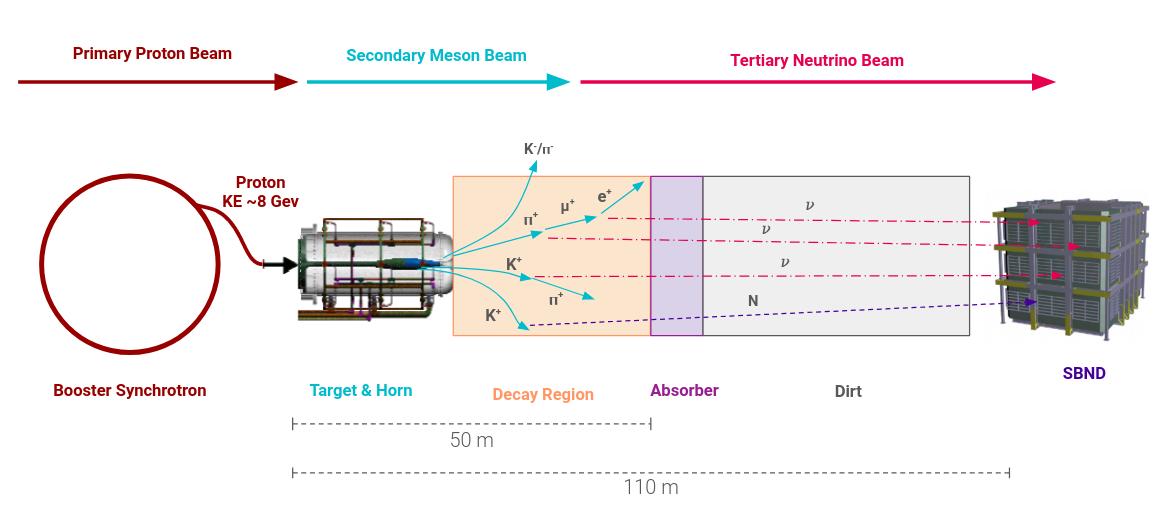
\includegraphics[width=1.0\textwidth]{BNBDiagram}
\caption[Particle Production in the Booster Neutrino Beam]{
Diagram showing the particle production in the BNB.
}
\label{fig:BNBDiagram}
\end{figure}

%beam simulation
%Explain what meson is in the flux, what tuning is used, 
The beam is simulated using GEANT4 with different tunings for the composition of the secondary mesons and hadrons produced from $p + Be$ interactions \cite{BNBMiniBooNE}.
The $\pi^{\pm}$ production is tuned to the HARP data set using Sanford-Wang parametrisation.
The $K^{+}$ production is extrapolated to the global $K^{+}$ production data using Feynman scaling-based parametrisation, and further constrained by SciBooNE's direct measurements of $K^{+}$ production from the BNB \cite{SciBooNE}. 
Other secondary hadrons and mesons such as $p$, $n$ and $K^{-}$ are modelled using the MARS hadronic interactions, however, their overall contribution to the neutrino flux is small. 
Interaction cross sections of $p/n + Be$ and $\pi^{\pm} + Be$ are also incorporated in flux predictions \cite{DavePhd}.
Uncertainties associated with the flux modelling are discussed in Section \ref{sec:signal_error}.
%The systematics uncertainties associated with the BNB flux are calculated by a re-weighting process, which will be presented in Chapter \ref{ChapterResult}.

Fig. \ref{fig:BNB_Meson_Flux} depicts the primary contributors to the secondary meson fluxes at the BNB, namely pions and kaons.
A small fraction of muons resulting from pion decays also contribute to the fluxes.
These fluxes are shown for the BNB operating in neutrino mode, mainly composed of positively charged mesons.
As discussed in Section \ref{sec2Production}, the flux of HNL comes from $K^{+}$ decays, which has energy peaking at $0.5 \sim 1$ GeV.
Ref \cite{BNBMiniBooNE} has highlighted significant uncertainties in the $K^{+}$ production cross sections within this energy range.
However, results from the SciBooNE experiment have demonstrated the validity of extrapolating higher energy $K^{+}$ data to the 1 GeV region using Feynman scaling \cite{SciBooNE}. 

\begin{figure}[hb!]
\begin{subfigure}{.5\linewidth}
\centering
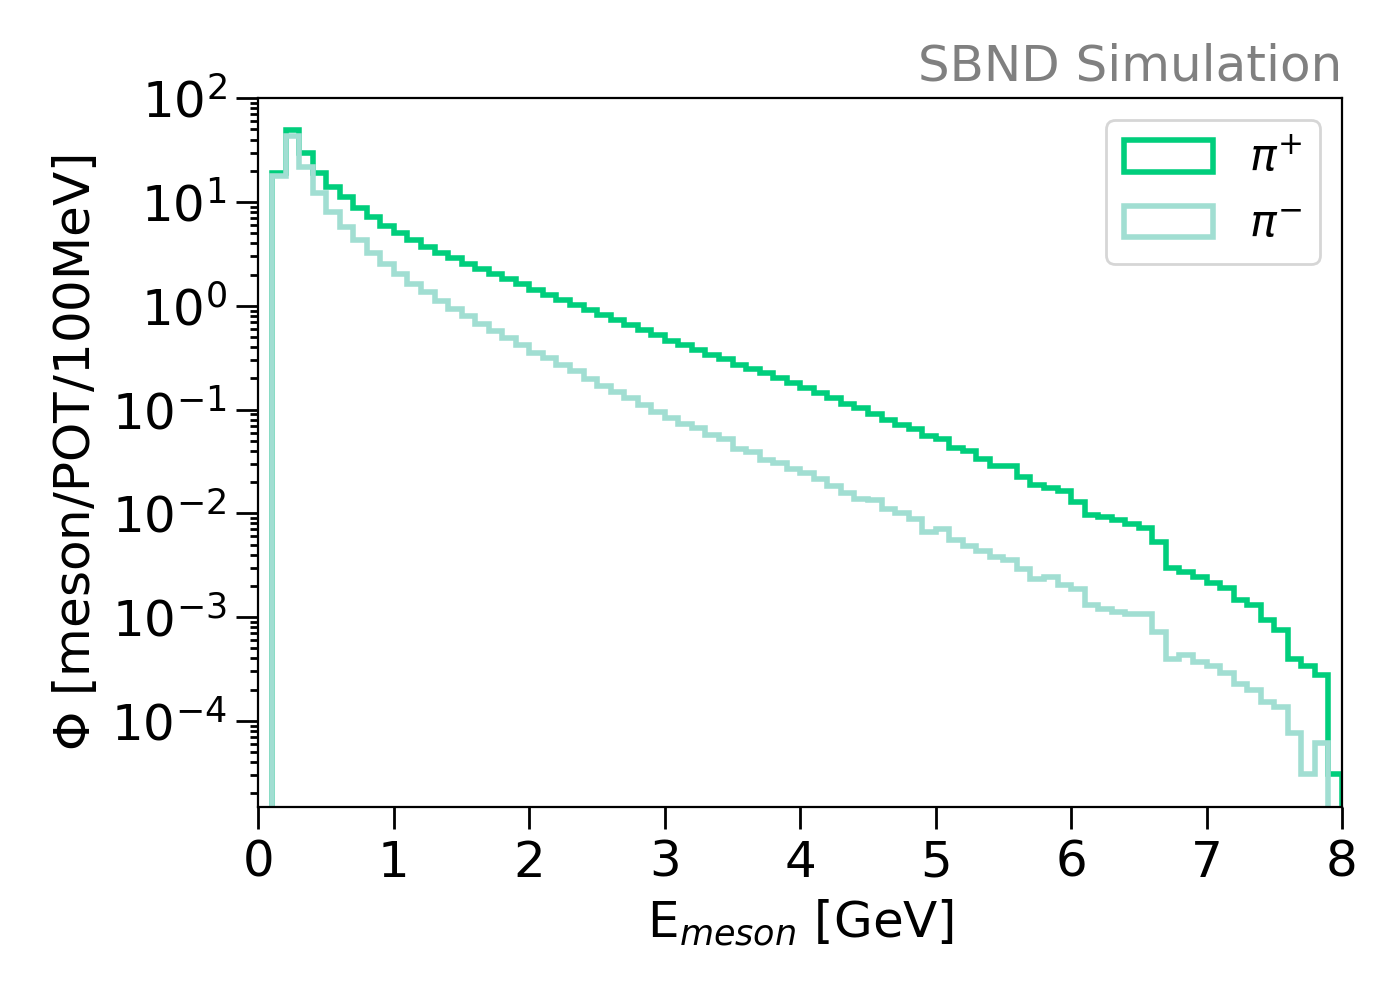
\includegraphics[width=1.0\textwidth]{BNB_Meson_Pion_Flux}
%\caption{}
%\label{fig:sub1}
\end{subfigure}%
\begin{subfigure}{.5\linewidth}
\centering
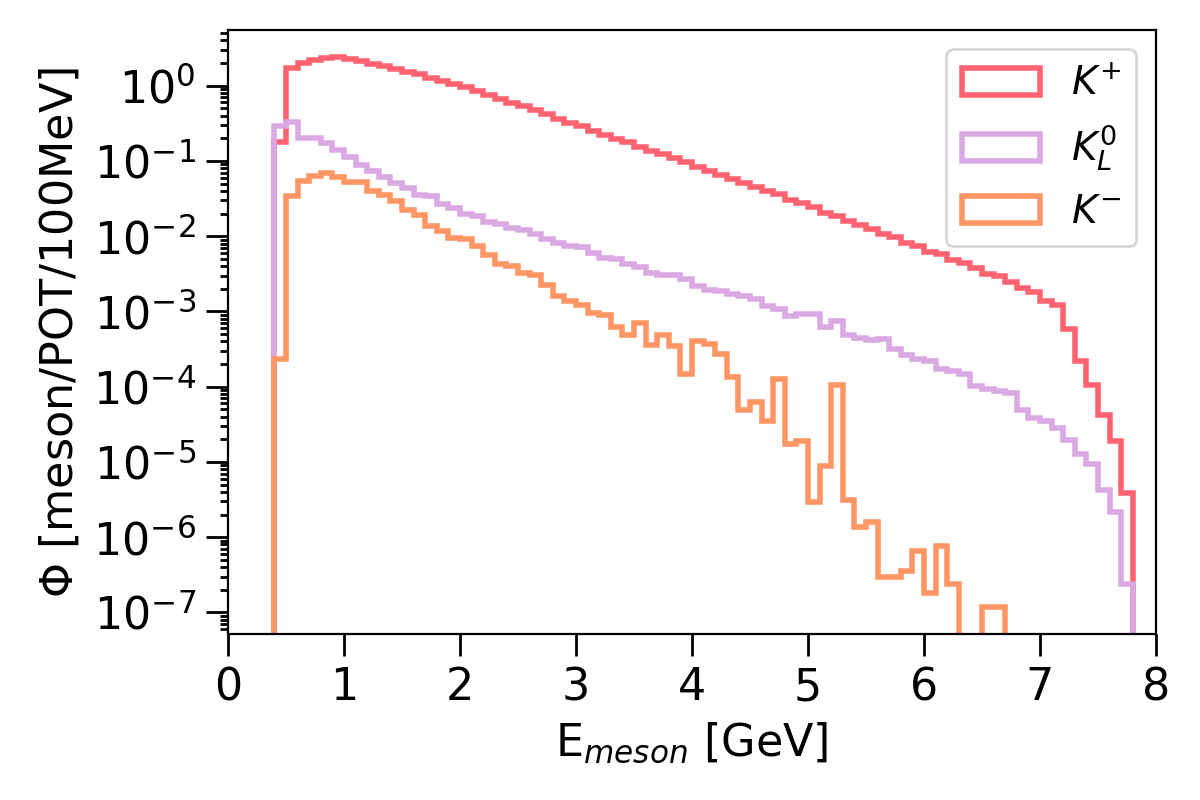
\includegraphics[width=1.0\textwidth]{BNB_Meson_Kaon_Flux}
%\caption{}
%\label{fig:sub2}
\end{subfigure}\\[1ex]
\begin{subfigure}{\linewidth}
\centering
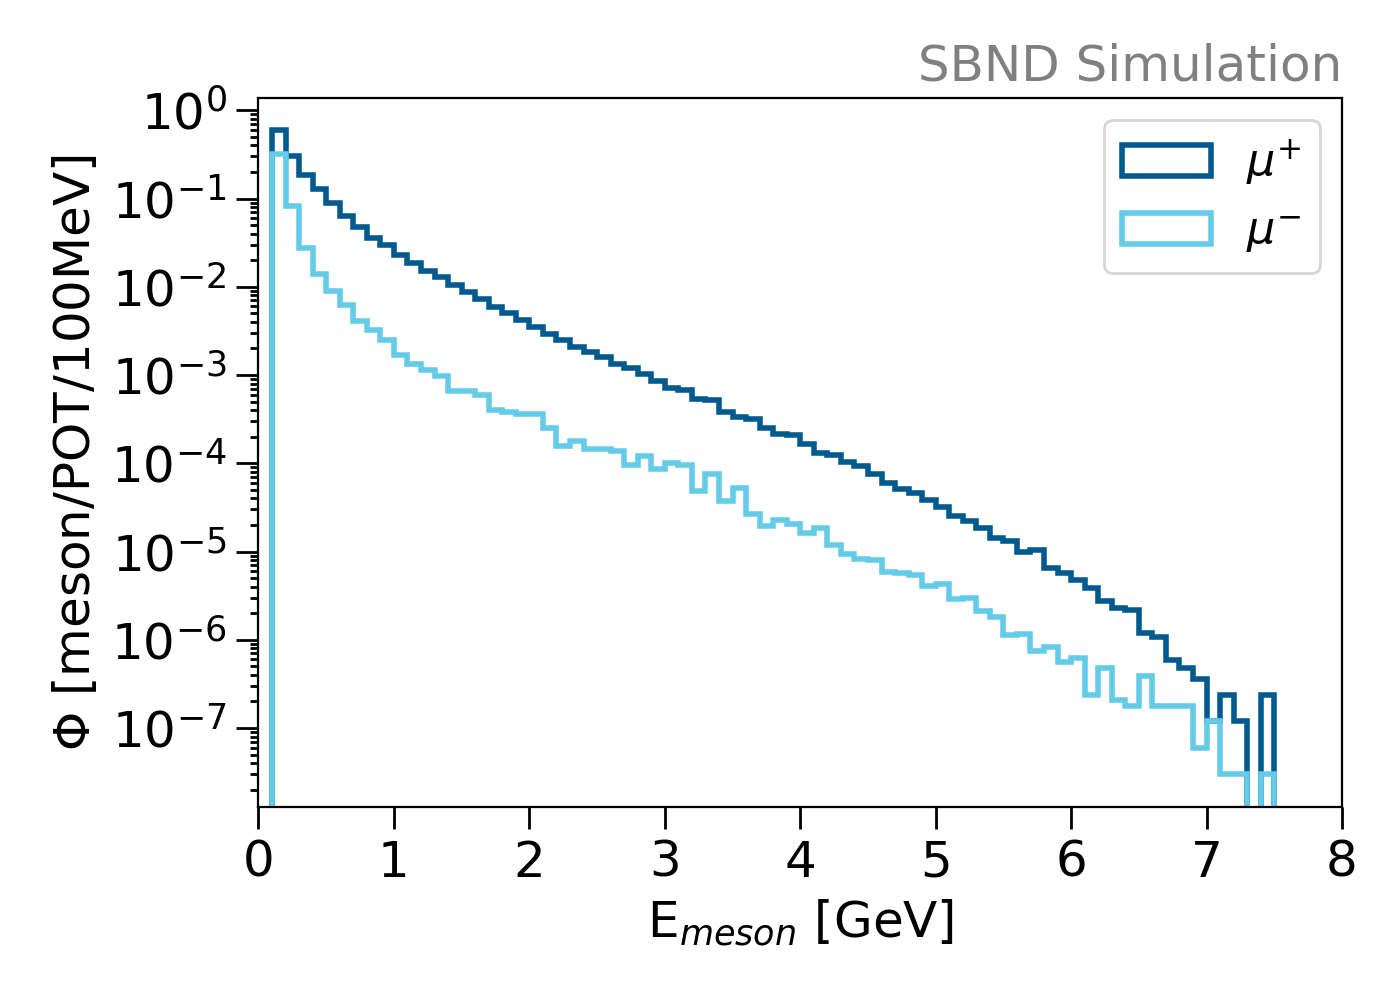
\includegraphics[width=0.5\textwidth]{BNB_Meson_Muon_Flux}
%\caption{}
%\label{fig:sub3}
\end{subfigure}
\caption[Simulated Fluxes of Secondary Mesons]{
Simulated fluxes for the secondary mesons produced in the BNB. 
}
\label{fig:BNB_Meson_Flux}
\vspace{0.5cm}
\end{figure}

The simulation of the neutrino flux at the front face of SBND is depicted in Fig. \ref{fig:BNB_combined_neutrino_flux}, shown for different flavours of neutrinos. 
The flux is predominantly composed of $\nu_{\mu}$ ($\sim90\%$), followed by $\bar{\nu}_{\mu}$ ($\sim9\%$), while the combination of $\nu_{e}$ and $\bar{\nu}_{e}$ contributes less than 1\%.
%Fig. \ref{fig:BNB_neutrino_flux} depicts the parent mesons for each neutrino flavour.
Pion production is the dominant mechanism for both $\nu_{\mu}$ and $\bar{\nu}_{\mu}$, followed by kaon and muon production. 
%Notably, a peak in the $\nu_{\mu}$ flux can be seen at half the mass of the kaon (235.5 MeV) resulting from kaon decay at rest \cite{kaonDecayNu}.
In the case of $\nu_{e}$, muons produced from pion decay are the primary source at low energies, while kaon production becomes the dominant mode at higher energies. 
Finally, $\bar{\nu}_{e}$ mainly originates from $K^{0}_{L}$ production.

\begin{figure}[hb!] 
\centering    
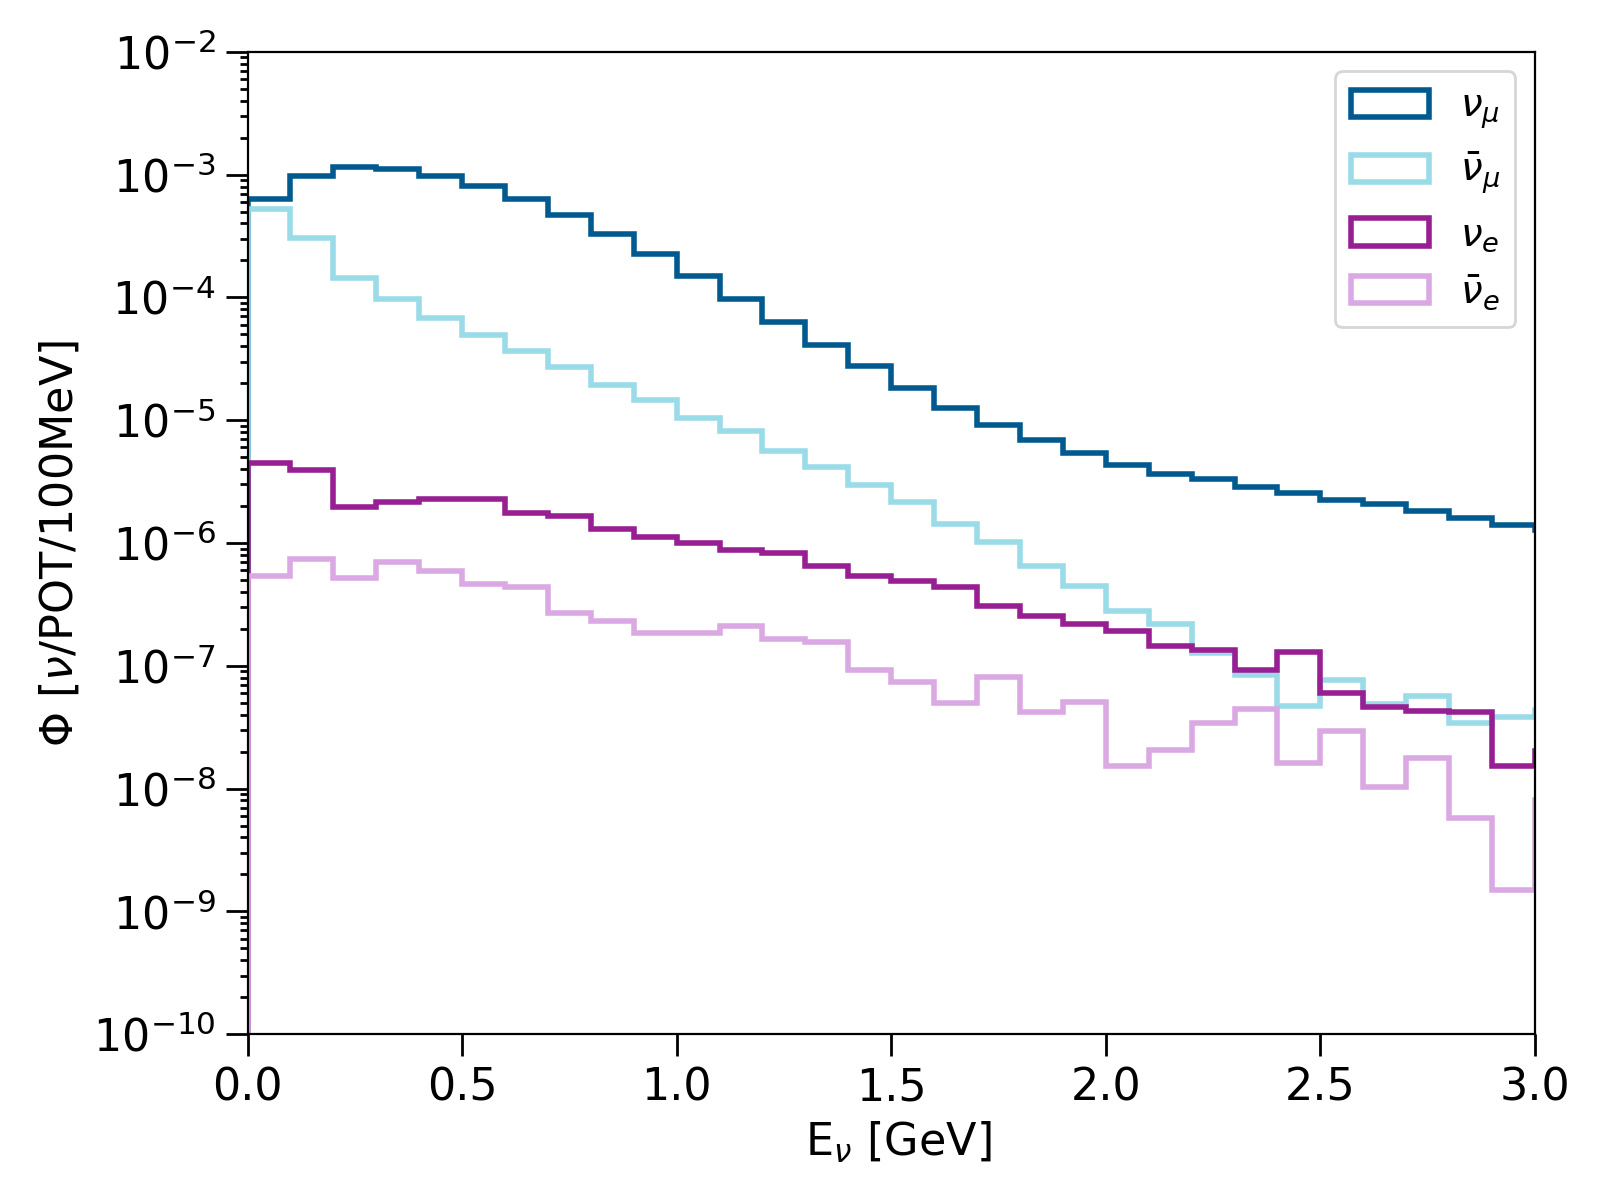
\includegraphics[width=0.5\textwidth]{BNB_combined_neutrino_flux}
\caption[Simulated Neutrino Fluxes at the Front Face of SBND]{
Simulated neutrino fluxes at the front face of SBND. 
}
\label{fig:BNB_combined_neutrino_flux}
\end{figure}

%\begin{figure}[h] 
%\vspace{0.5cm}
%\centering    
%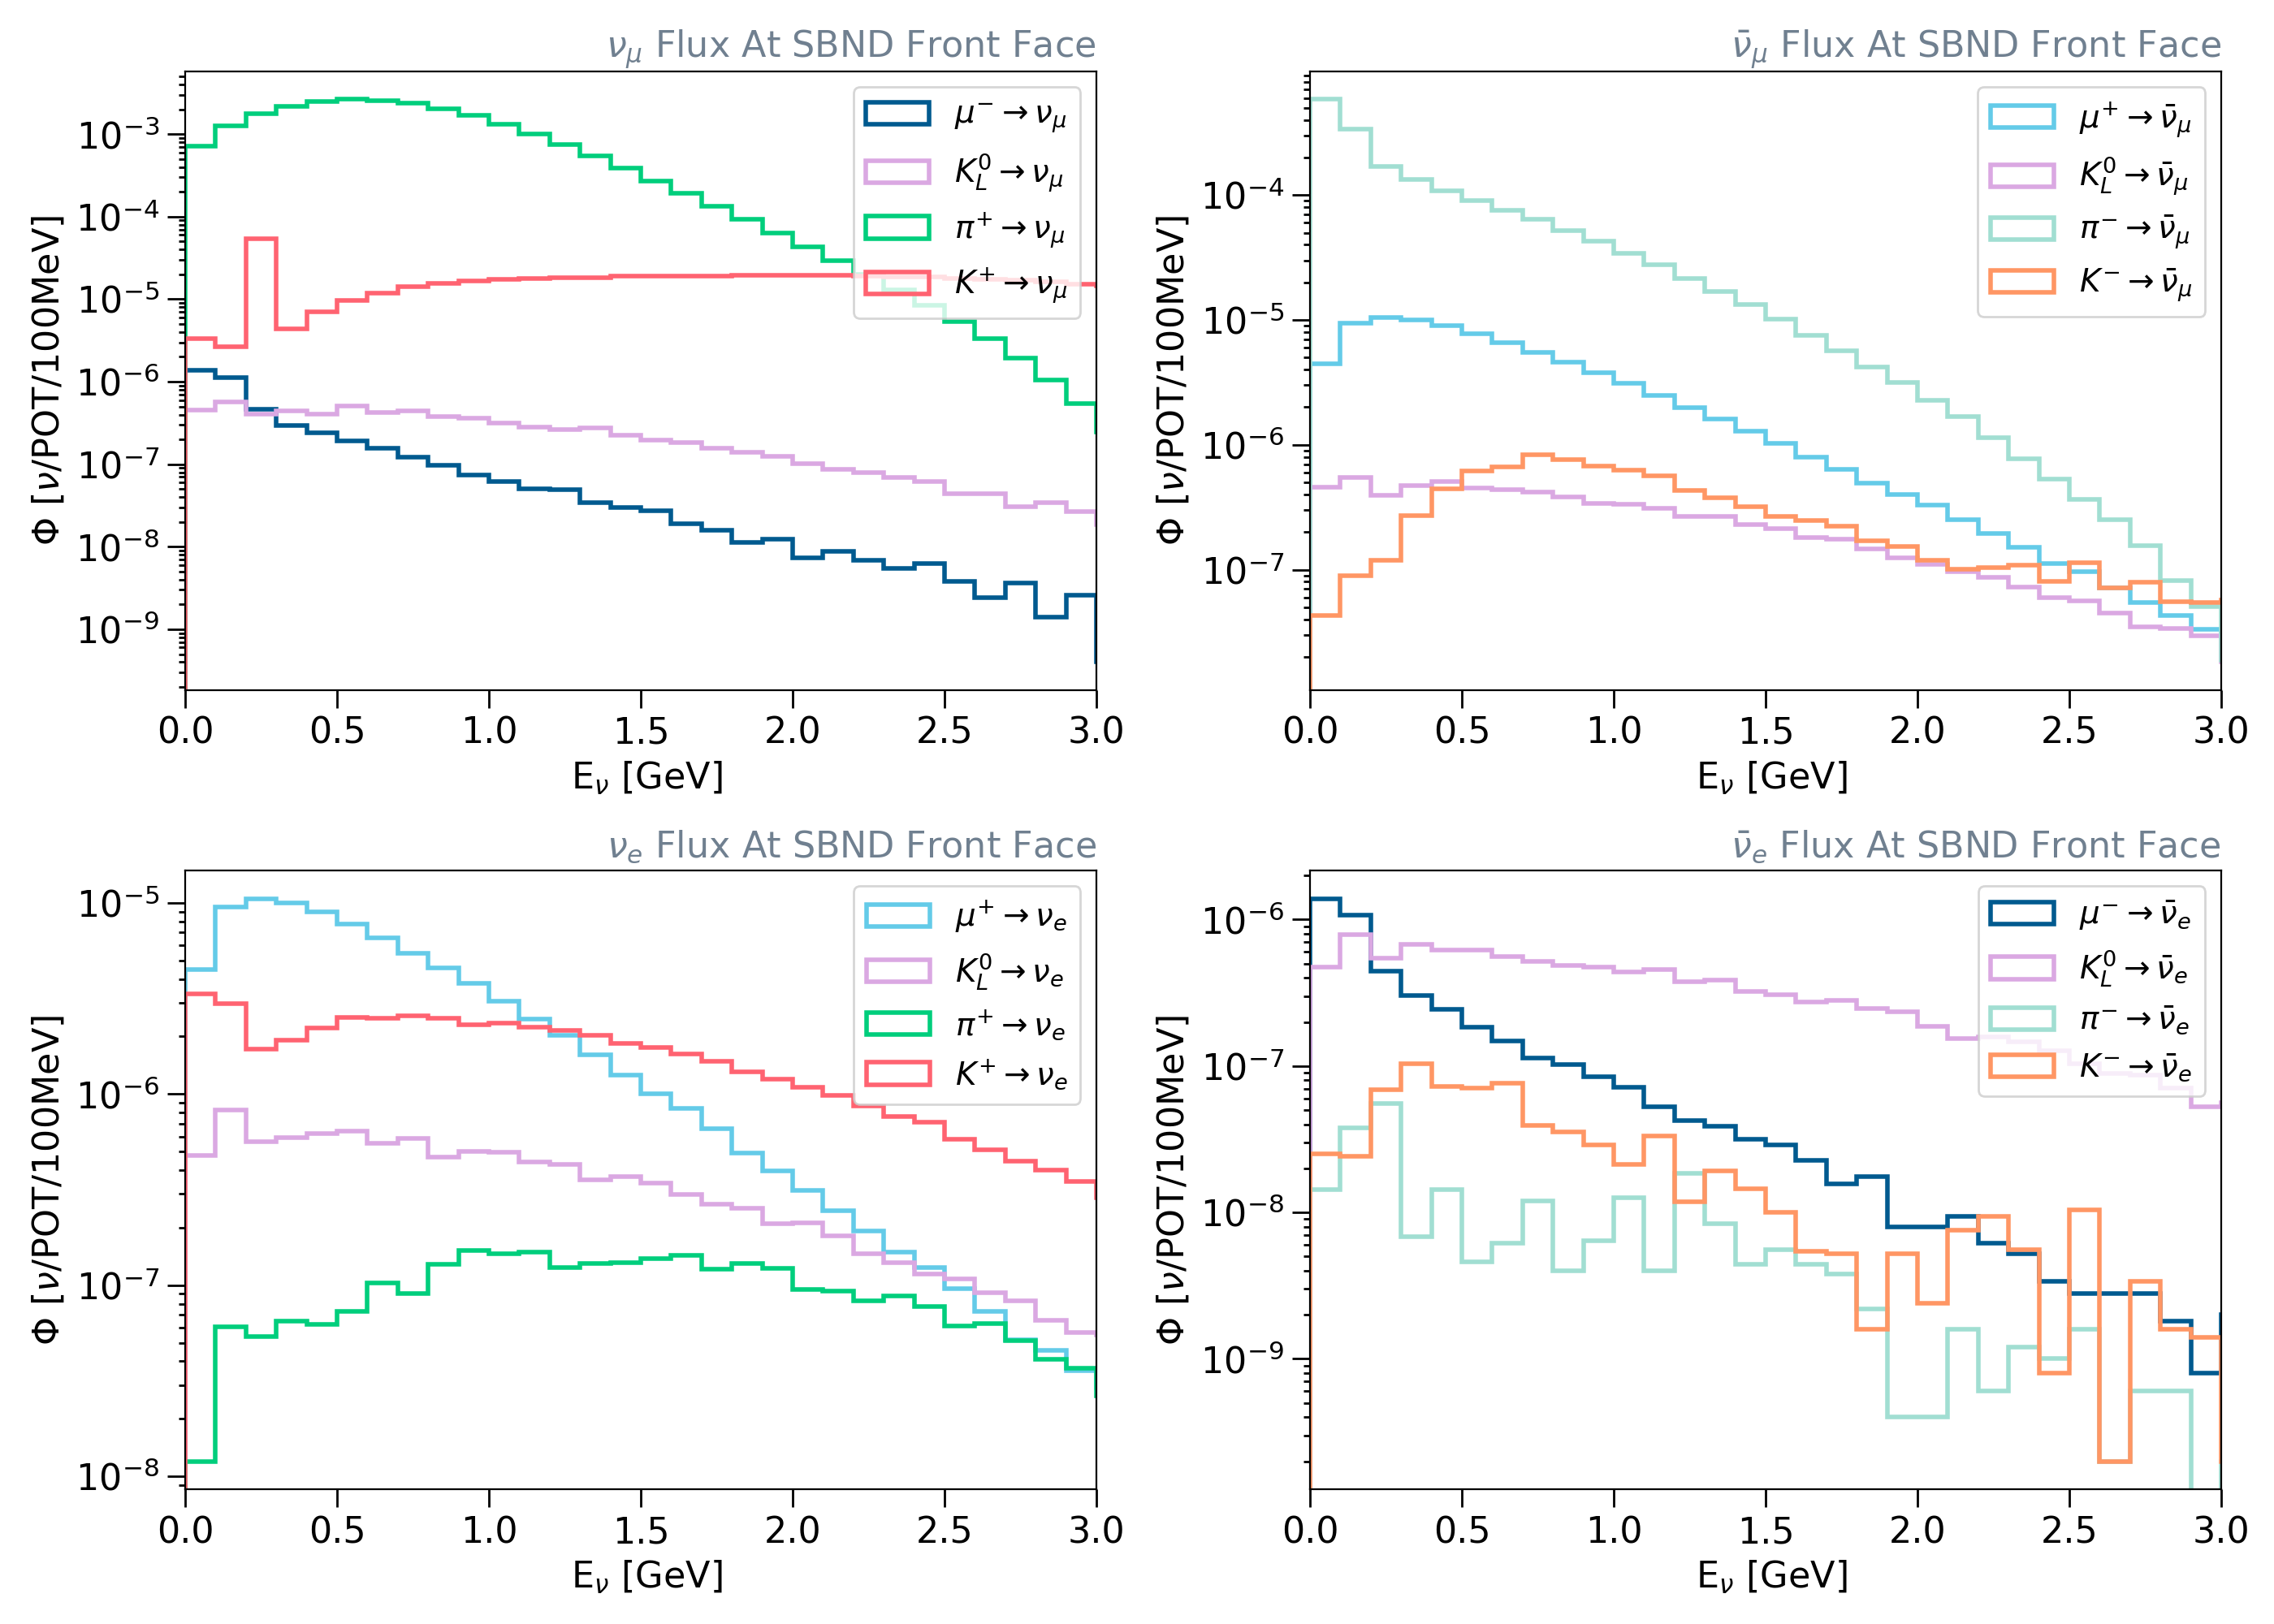
\includegraphics[width=1.0\textwidth]{BNB_neutrino_flux}
%\caption[Simulated Neutrino Fluxes of Different Flavours at the Front Face of SBND]{
%Simulated fluxes of different neutrino flavours at the front face of SBND, broken down into types of parent mesons.
%}
%\label{fig:BNB_neutrino_flux}
%\end{figure}

%********************************** %First Section  **************************************
\section{Concluding Remarks}
\label{sec:sbnd_conclude}

SBND, together with other experiments in the SBN program, aims to conclusively address the low energy excess observed by LSND, MiniBooNE, and other nuclear reactor and solar neutrino experiments. 
SBND will play a crucial role in constraining systematic uncertainties by measuring large statistics of the unoscillated neutrino flux from the BNB.
Additionally, SBND has a rich physics program covering high precision $\nu$-Ar cross section measurements and searches for BSM physics. 
Of particular relevance to this thesis, SBND aims to establish competitive limits on the coupling of HNLs within the probable mass range from the BNB.

The hardware of SBND comprises three detection subsystems: the TPC, the PDS, and the CRT system, alongside the hardware triggering subsystem. 
Each of these subsystems has dedicated readout electronics, which are managed by a complex DAQ subsystem.
SBND measures the flux coming from the BNB, which has a distinctive bucket structure that can be resolved with a sufficient timing resolution. 
This feature can be exploited in the search for HNLs at SBND since being massive results in HNLs arriving late relative to the bucket structure of SM neutrinos. 
Chapter \ref{ChapterSim} provides a description of the simulation framework at SBND to enable the exploration of the detector physics capabilities in the BSM regime using Monte Carlo.  

%The event building process of the DAQ relies on the timing information acquired from each subsystem. 
%This process assembles the foundation of physics event upon which low-level and high-level reconstructions are built to achieve nanosecond timing resolution.
%The timing characterisation of the readout electronics will be discussed in the forthcoming chapter.
